\documentclass{beamer}

\usepackage{graphicx}
\usepackage{listings}
\usepackage[utf8]{inputenc}
\usepackage{tikz}
\usetikzlibrary{calc}
\usetikzlibrary{intersections}

%30 min

\lstset{
  basicstyle=\footnotesize,        % the size of the fonts that are used for the code
  breakatwhitespace=true,         % sets if automatic breaks should only happen at whitespace
  breaklines=true,                 % sets automatic line breaking
  commentstyle=\color{green},      % comment style
  keywordstyle=\color{blue},       % keyword style
  language=C++,                    % the language of the code
  numbers=none,                    % where to put the line-numbers; possible values are (none, left, right)
}


\newcommand{\sectiontitle}[1]{
    \section{#1}
    \begin{frame}
        \centering
        \LARGE{#1}
    \end{frame}
}
\newcommand{\subsectiontitle}[1]{
    \subsection{#1}
    \begin{frame}
        \LARGE{#1}
    \end{frame}
}

\newcommand{\inlinecpp}[1]{
    \lstinline[language=C++]{#1}
}


\title[ugtest]{ugtest}
\author{Tobias Trautmann}
\institute{GCSC}

\begin{document}

    \begin{frame}
        \titlepage
    \end{frame}

    \begin{frame}{Outline}
        \tableofcontents
    \end{frame}


    \sectiontitle{Introduction to testing}
        %talk about differneces between debugging and testing
        %talk about coverage and ease of defect localistion
        %systematisch!!
        %tooling
        %nicht so viel theorie!!!
        \subsection{Goals}
        \begin{frame}{Goals of testing}
           %nur geteste software erzeugt wert
           %it := Software
           \begin{itemize}
               \item check wether it meets requirements\pause
               \item check if it performs its functions within an acceptable time\pause
               \item make it sufficiently usable\pause
               \item can be run in its intended environments\pause%rephrase
               \item increase trust in its results\pause
               \item make code maintainable\pause
               \item make code refactorable
           \end{itemize}
           \Large{$\Rightarrow$ Testing software is a \textbf{necessity}}
        \end{frame}

        \subsectiontitle{Definitions}
        \begin{frame}{Defects}
            %make an explanation why definition of failure is importat
            %makes it much easier to understand bugs during debugging and
            %allows to set priorities when developing test cases
            %HELP
            Where do defects come from?\\
            Prioritize defects\\
            Are you responsible for it?\\
            mitigation
            \begin{tabular}{c|c|c}
                bug in code   & integration & error in design \\
            \end{tabular}
        \end{frame}

        \begin{frame}{Definition of done}
            %besonderer anwendungsfall geplante fluktuation (studenten kommen und gehen)
            %code coverage
            %HELP
            \begin{itemize}
                \item Code
                \begin{itemize}
                    \item 
                \end{itemize}

                \item Tests
                \begin{itemize}
                    \item Coverage
                \end{itemize}

                \item Documentation
                \begin{itemize}
                    \item User
                    \item Maintainer
                \end{itemize}
            \end{itemize}
        \end{frame}
        %%WHAT DO I TEST?!!!!!!!!!!!!!!!!!!!!!!!!!!!!!!
        \subsection{Efficency}
        \begin{frame}{Efficency}
            %Talk about each test level, what it does what its for and when to do them
            %effort goes up with pyramid
            %time to develop goes up
            % pesticide paradox\\%bugs become more subtle the more you cover
            % testen für qualität nicht für statistik!!
            % amount of work put into testing 25\%-50\% of total  time!!!!!
            \centering
            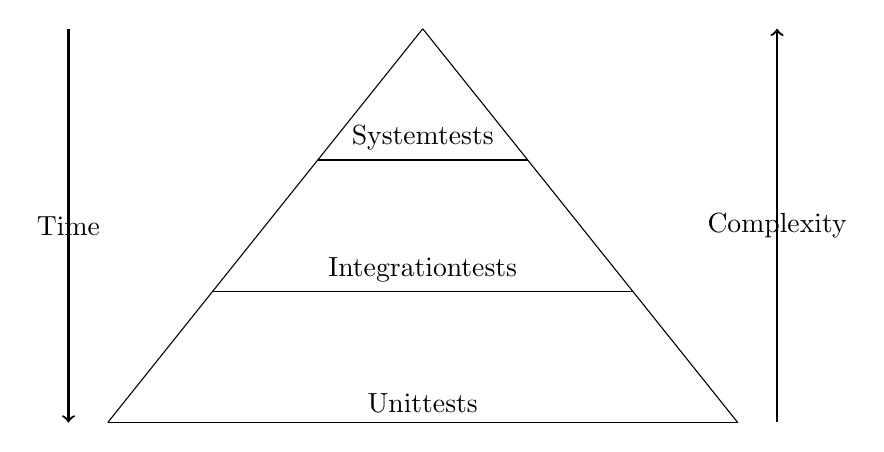
\begin{tikzpicture}
                \coordinate (A) at (-4,-1) {};
                \coordinate (B) at ( 4,-1) {};
                \coordinate (C) at (0,4) {};
                \draw[name path=AC] (A) -- (C);
                \draw[name path=BC] (B) -- (C);
                \draw[name path=AB] (A) -- (B);
    
                \foreach \y/\A in {0/Unittests,1/Integrationtests,2/Systemtests} {
                    \draw ($(A)!\y/3!(C)$) -- ($(B)!\y/3!(C)$) node[midway,above] {\A};\pause
                }
                \draw[thick, ->] (-4.5,4) -- (-4.5, -1) node[midway] {Time};\pause
                \draw[thick, <-] (4.5,4) -- (4.5, -1) node[midway] {Complexity};
            \end{tikzpicture}
        \end{frame}

        \subsectiontitle{Approaches}%HELP
        \begin{frame}{Continous Integration / Continous Delivery}%Do i want to present this??
            \centering
            \begin{figure}
                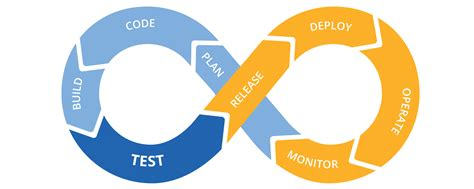
\includegraphics[width=12cm]{./images/cicd.jpeg}
            \end{figure}
            % https://www.mabl.com/hubfs/CICDBlog.png\\
            % https://www.mabl.com/blog/what-is-cicd\\
            % https://en.wikipedia.org/wiki/Continuous_delivery\\
            % https://en.wikipedia.org/wiki/Continuous_integration\\
            % https://www.mabl.com/blog/what-is-cicd
        \end{frame}

        \begin{frame}{Test driven development}
            \centering
            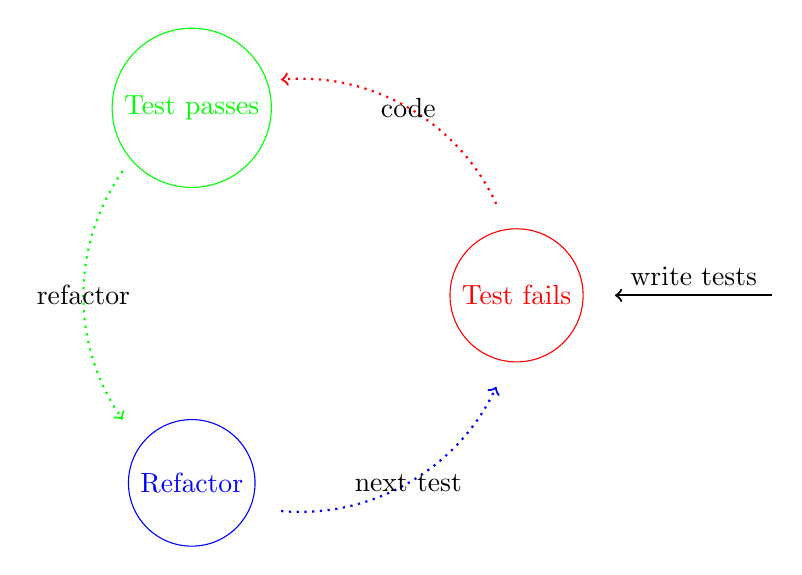
\begin{tikzpicture}
                \def \n {3}
                \def \radius {2.75cm}
                \def \margin {25}
                \draw[<-,thick] (4,0) -- (6,0) node[midway, above] {write tests};
                \foreach \s/\A/\C/\D in {1/Test fails/red/code, 2/Test passes/green/refactor, 3/Refactor/blue/next test}
                {
                    \node[draw, circle,\C] at ({360/\n * (\s - 1)}:\radius) {\A};\pause
                    \draw[->, dotted, thick, \C] ({360/\n * (\s - 1)+\margin}:\radius) arc ({360/\n * (\s - 1)+\margin}:{360/\n * (\s)-\margin}:\radius) node[midway, black] {\D};
                }
            \end{tikzpicture}
        \end{frame}


    \sectiontitle{Boost.Test}

        \subsection{Basic usage}
        \begin{frame}{Structure}
            \lstinputlisting[language=c++]{scripts/structure.cpp}
        \end{frame}

        \begin{frame}{Assertion Levels}
            \begin{tabular}{c|c|c}
                assertion level &   error counter   &   test continuation   \\
                \hline
                warn    &       &   yes  \\
                check   &   ++  &   yes \\
                require &   ++  &   no  \\
            \end{tabular}
        \end{frame}

        % \begin{frame}{Basic Checks}
        %     \begin{itemize}
        %         \item  \inlinecpp{BOOST_<level>(predicate)}
        %         \item  \inlinecpp{BOOST_<level>_<GE,LE,GT,LT,NE>(left, right)}
        %         \item  \inlinecpp{BOOST_<level>_EQUAL(left, right)}
        %         \item  \inlinecpp{BOOST_IS_DEFINED(SYMBOL)}
        %     \end{itemize}
        % \end{frame}
        % \begin{frame}{Warn}
        %     \lstinputlisting[language=c++]{scripts/basic_warn.cpp}
        % \end{frame}
        % \begin{frame}{Check}
        %     \lstinputlisting[language=c++]{scripts/basic_checks.cpp}
        % \end{frame}
        % \begin{frame}{Require}
        %     \lstinputlisting[language=c++]{scripts/basic_require.cpp}
        % \end{frame}

        \begin{frame}{Float point comparison}
            \lstinputlisting[language=c++]{scripts/floatpoint_comparison.cpp}
        \end{frame}

        \begin{frame}{Exception handling}
            \lstinputlisting[language=c++]{scripts/exception_handling.cpp}      
        \end{frame}

        \subsection{Fixtures}
        \begin{frame}[plain]{Fixtures}
            \lstinputlisting[language=C++]{scripts/fixtures.cpp}
        \end{frame}

        \subsection{Templates}
        \begin{frame}[plain]{Templates}
            \lstinputlisting[language=C++]{scripts/templates.cpp}
        \end{frame}

    \sectiontitle{Testing}
        \subsection{Test executable}
        \begin{frame}{Test execution}
            \begin{itemize}
                \item add buildflags "--fprofile-arcs --ftest-coverage --fPIC" as well as no optimization for code coverage analysis
                \item build ug with UGTest and your plugin activated
                \item your plugin contains tests in a top level folder named "tests"
                \item executable named "ugtest\_unit" and "ugtest\_system" lands in ug4/bin
                \item \href{https://www.boost.org/doc/libs/1_58_0/libs/test/doc/html/utf/user-guide/runtime-config/reference.html}{list of params}
                \item example: \lstinline[language=bash]{ug4/bin $ ./ugtest_unit --log-level=ALL --log-format=HRF}
                \item Show result
            \end{itemize}
        \end{frame}
        
        \subsection{Jenkins}
        \begin{frame}{Automatization with Jenkins}
            \begin{itemize}
                \item Cobertura
                \item two builds one serial, one parallel -> two test runs
                \item Code coverage: gcovr can produce xml for cobertura
                \item needs log\_format=XML
            \end{itemize}
        \end{frame}

        \subsection{Docker}
        \begin{frame}{Automatization with Docker}
            \begin{itemize}
                \item Container stuff
                \item \href{https://github.com/Tobias-Trautmann/docker4ug4}{Dockerfile}
            \end{itemize}
        \end{frame}

    \section{Additional resources}
    \begin{frame}{Additional resources}
            \begin{itemize}
                \item \href{https://www.boost.org/doc/libs/1_58_0/libs/test/}{Boost.Test 1.58 documentation}
                \item \href{https://github.com/UG4/plugin_UGTest}{ugtests github}
                \item Antipatterns
                \item \href{https://docs.docker.com/}{Docker Documentation}
                \item \href{https://www.boost.org/doc/libs/1_73_0/libs/test/}{newest Boost.Test} %(often better documentation of already existing features)
                \item Concept stuff for software development
            \end{itemize}
    \end{frame}

    \section{Refereneces}
    \begin{frame}{References}
        \begin{itemize}
            \item \href{https://en.wikipedia.org/wiki/Software_testing}{wiki}
            %definitly wrong pls fix
            \item Basiswissen Softwaretest
        \end{itemize}
    \end{frame}
\end{document}